%%%%%%%%%%%%%%%%%%%%%%%%%%%%%%%%%%%%%%%%%
% University of Newcastle report
% LaTeX Template
% Version 1.0 (20/2/19)
%
% This template has been downloaded from:
% http://www.LaTeXTemplates.com
%
% Original author:
% WikiBooks (http://en.wikibooks.org/wiki/LaTeX/Title_Creation)
% Modified by Elsa Slattegard to fit Uppsala university
% Modified by Alex Mendes to fit University of Newcastle
% License:
% CC BY-NC-SA 3.0 (http://creativecommons.org/licenses/by-nc-sa/3.0/)

%\title{Title page with logo}
%----------------------------------------------------------------------------------------
%	PACKAGES AND OTHER DOCUMENT CONFIGURATIONS
%----------------------------------------------------------------------------------------

\documentclass[12pt]{article}
\usepackage[english]{babel}
\usepackage[utf8x]{inputenc}
\usepackage{amsmath}
\usepackage{graphicx}
\usepackage[export]{adjustbox}
\usepackage{natbib}
\usepackage{float}
\usepackage[colorinlistoftodos]{todonotes}
\usepackage{rotating}
\usepackage{tikz}
\usepackage[
    breaklinks=true,
    allbordercolors=blue,
    colorlinks=true,
    anchorcolor=black,
    citecolor=black,
    filecolor=black,
    linkcolor=black,
    menucolor=black,
    runcolor=black,
    urlcolor=blue,
    linktoc=all
]{hyperref}

\usepackage{geometry}
\usepackage{hyperref}

\usepackage[nottoc,numbib]{tocbibind}

\bibliographystyle{agsm}

\begin{document}

\begin{titlepage}

\newcommand{\HRule}{\rule{\linewidth}{0.5mm}} % Defines a new command for the horizontal lines, change thickness here

\center % Center everything on the page

%----------------------------------------------------------------------------------------
%	HEADING SECTIONS
%----------------------------------------------------------------------------------------

\textsc{\LARGE The University of Newcastle}\\[0.5cm]
\textsc{\large School of Electrical Engineering and Computing}\\[1.0cm] % Name of your university/college

\includegraphics[scale=.3]{images/uon-logo-square.png}\\[1cm] % Include a department/university logo - this will require the graphicx package
\textsc{\LARGE Advanced Databases}\\[0.5cm] % Major heading such as course name
\textsc{\large COMP3350 - Semester 1, 2020}\\[0.5cm] % Minor heading such as course title

%----------------------------------------------------------------------------------------
%	TITLE SECTION
%----------------------------------------------------------------------------------------

\HRule \\[0.4cm]
{ \huge \bfseries Item Sales and Ordering Patterns}\\[0.4cm] % Title of your document
\HRule \\[1.5cm]

%----------------------------------------------------------------------------------------
%	AUTHOR SECTION
%----------------------------------------------------------------------------------------

\begin{minipage}{1.0\textwidth}
\begin{flushleft} \large
\emph{Author:}\\

Karl \textsc{Foley}\\ % Student 1
Dillon \textsc{Latimore}\\ % Student 2
\end{flushleft}

\end{minipage}\\[2cm]

% If you don't want a supervisor, uncomment the two lines below and remove the section above
%\Large \emph{Author:}\\
%John \textsc{Smith}\\[3cm] % Your name

%----------------------------------------------------------------------------------------
%	DATE SECTION
%----------------------------------------------------------------------------------------

{\large \today}\\[2cm] % Date, change the \today to a set date if you want to be precise

\vfill % Fill the rest of the page with white space

\end{titlepage}

%----------------------------------------------------------------------------------------
%	TABLE OF CONTENTS
%----------------------------------------------------------------------------------------

% Create table of contents
\setcounter{page}{1}
\pagenumbering{roman}
\tableofcontents
\newpage
\listoffigures
\newpage

% Set the page number to 1
\setcounter{page}{1}
\pagenumbering{arabic}

\section{Introduction}

\subsection{DashBoards}
\begin{flushleft}
This report explores the buying tends of WW1's customers by year. The data is presented in two different dashboards. The first dashboard is the item Sales Dashboard, this looks at most bought items, the amount of items by region, along side profit per item and the total dollar revenue amount sold for an item. The Last 3 diagrams only look at the top ten items for either respective view.
\vfill
The second dashboard is the item Purchase DashBoard, This looks at most Purchased items, most purchased items by Supplier, Suppliers and corresponding post codes and the volume of purchases by month.
\vfill
For further Drill downs of each of these metrics Refer to the dashboard in power BI for a closer look at each item.
\end{flushleft}

\subsection{Limitations}
\begin{flushleft}
    When comparing where WW1 customers are and where WW1 Suppliers are we are unable to compare the two because data provided for supplies location are a postcode which is not a dataset of the cities dimension given to us by WW1.
\end{flushleft}


\section{Item Sales Tends by Year}

\begin{flushleft}
    For Items Sales charts are all on a year specific Dashboard- 2013 figure: \ref{Item Sales 2013 DashBoard}, 2014 figure: \ref{Item Sales 2014 DashBoard}, 2015 figure: \ref{Item Sales 2015 DashBoard} and 2016 figure: \ref{Item Sales 2016 DashBoard}.
\end{flushleft}

\subsection{Stock Items By Sales Count}

\begin{flushleft}
Looking a each year's items by the quantity that are sold, refer to 2013 figure: \ref{Stock item by Sale Count 2013}, 2014 figure: \ref{Stock item by Sale Count 2014}, 2015 figure: \ref{Stock item by Sale Count 2015} and 2016 figure: \ref{Stock item by Sale Count 2016}. Starts to show a that there is no trend popular items over the four years of data. The top 10 items that WW1 ships per year based on quantity are not the same. There is only one recurring item across all items which is the "DBA Joke mug - it depends (white)". In the past 2 years "10 mm Static Bubble Wrap (blue) 10m" has appeared apeared in the top 10. The top 10 items per quantity year over year tends be about the same quantity. With only having 5 months of data for 2016, the trend that the most popular items for WW1 will have a quantity between 300-400 items looks to be on track.
\end{flushleft}

\subsection{Items By Total Sales}
\begin{flushleft}
Exploring the Data year over year for Items by total sales price, refer to 2013 figure: \ref{Total Sales by item 2013}, 2014 figure: \ref{Total Sales by item 2014}, 2015 figure: \ref{Total Sales by item 2015} and 2016 figure: \ref{Total Sales by item 2016}.. Shows that the same items show up. With further exploration of these items there is a combination of factors why these items show up. The leading factor is item price, these items year over year sell about the same quantity which is why the items move around in the top 10.

\end{flushleft}

\subsection{Items Ordered by State}
\begin{flushleft}
Stuff

\end{flushleft}

\subsection{Item By Sales Territories}
\begin{flushleft}
Stuff

\end{flushleft}

\subsection{Profit by Item}
\begin{flushleft}
Stuff

\end{flushleft}

\section{Item Purchase Tends by Year}

\begin{flushleft}
    For Items purchased charts are all on a year specific Dashboard - 2013 figure: \ref{Item Purchase 2013 DashBoard}, 2014 figure: \ref{Item Purchase 2014 DashBoard}, 2015 figure: \ref{Item Purchase 2015 DashBoard} and 2016 figure: \ref{Item Purchase 2016 DashBoard}.
\end{flushleft}

\subsection{2013}
\begin{flushleft}
Stuff

\end{flushleft}

\subsection{2014}
\begin{flushleft}
Stuff

\end{flushleft}

\subsection{2015}
\begin{flushleft}
Stuff

\end{flushleft}

\subsection{2016}
\begin{flushleft}
Stuff

\end{flushleft}

\section{Conclusions and Recommendations}
\begin{flushleft}
Stuff

\end{flushleft}
\section{Appendix}
\appendix
\begin{figure}[H]
    \centering
    \includegraphics[width=18.5cm, angle=90]
    {images/Item sales2013.pdf}
    \caption{Item Sales 2013 DashBoard}
    \label{Item Sales 2013 DashBoard}
\end{figure}
\begin{figure}[H]
    \centering
    \includegraphics[width=18.5cm, angle=90]
    {images/Item sales2014.pdf}
    \caption{Item Sales 2014 DashBoard}
    \label{Item Sales 2014 DashBoard}
\end{figure}
\begin{figure}[H]
    \centering
    \includegraphics[width=18.5cm, angle=90]
    {images/Item sales2015.pdf}
    \caption{Item Sales 2015 DashBoard}
    \label{Item Sales 2015 DashBoard}
\end{figure}
\begin{figure}[H]
    \centering
    \includegraphics[width=18.5cm, angle=90]
    {images/Item sales2016.pdf}
    \caption{Item Sales 2016 DashBoard}
    \label{Item Sales 2016 DashBoard}
\end{figure}

\begin{figure}[H]
    \centering
    \includegraphics [width=17.5cm]
    {images/Sales/stock item by Sale Count2013.png}
    \caption{Stock item by Sale Count 2013}
    \label{Stock item by Sale Count 2013}
\end{figure}

\begin{figure}[H]
    \centering
    \includegraphics [width=17.5cm]
    {images/Sales/stock item by Sale Count2014.png}
    \caption{Stock item by Sale Count 2014}
    \label{Stock item by Sale Count 2014}
\end{figure}

\begin{figure}[H]
    \centering
    \includegraphics [width=17.5cm]
    {images/Sales/stock item by Sale Count2015.png}
    \caption{Stock item by Sale Count 2015}
    \label{Stock item by Sale Count 2015}
\end{figure}
\begin{figure}[H]
    \centering
    \includegraphics [width=17.5cm]
    {images/Sales/stock item by Sale Count2016.png}
    \caption{Stock item by Sale Count 2016}
    \label{Stock item by Sale Count 2016}
\end{figure}

\begin{figure}[H]
    \centering
    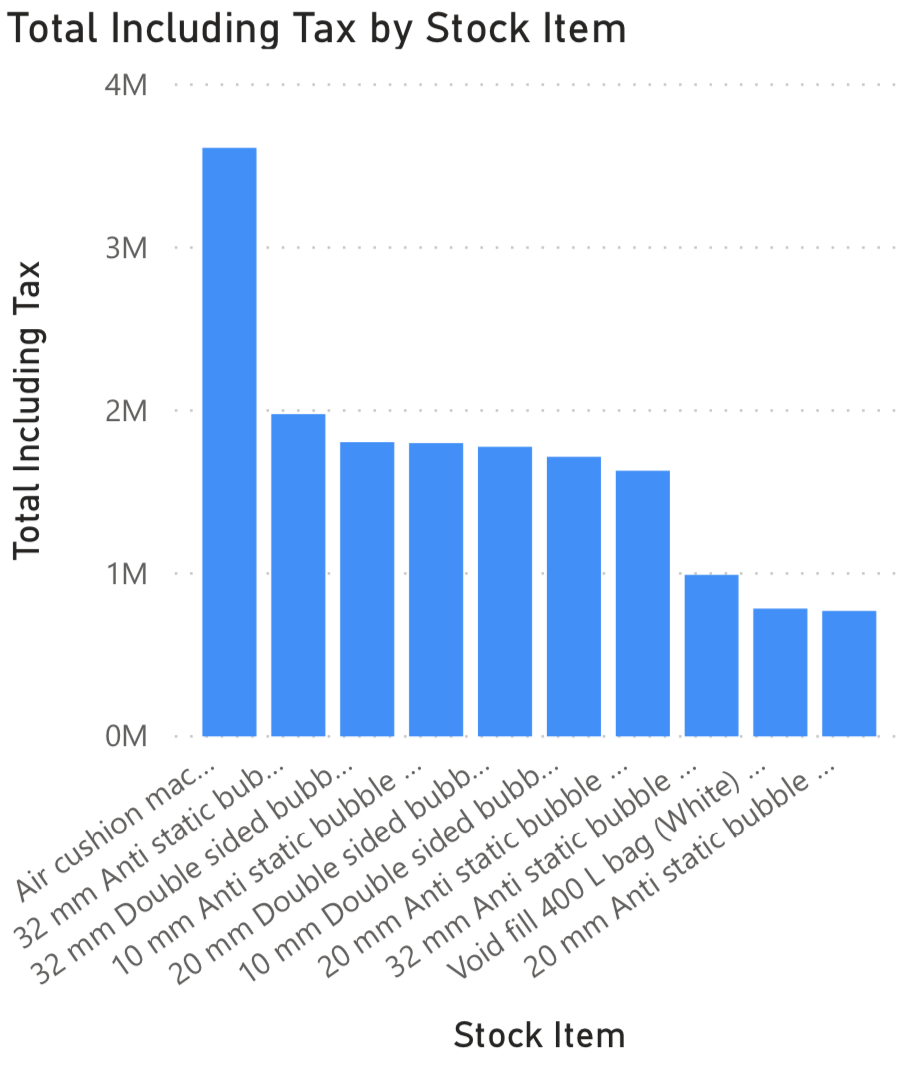
\includegraphics
    {images/Sales/Total Sales By stock item2013.png}
    \caption{Total Sales by item 2013}
    \label{Total Sales by item 2013}
\end{figure}

\begin{figure}[H]
    \centering
    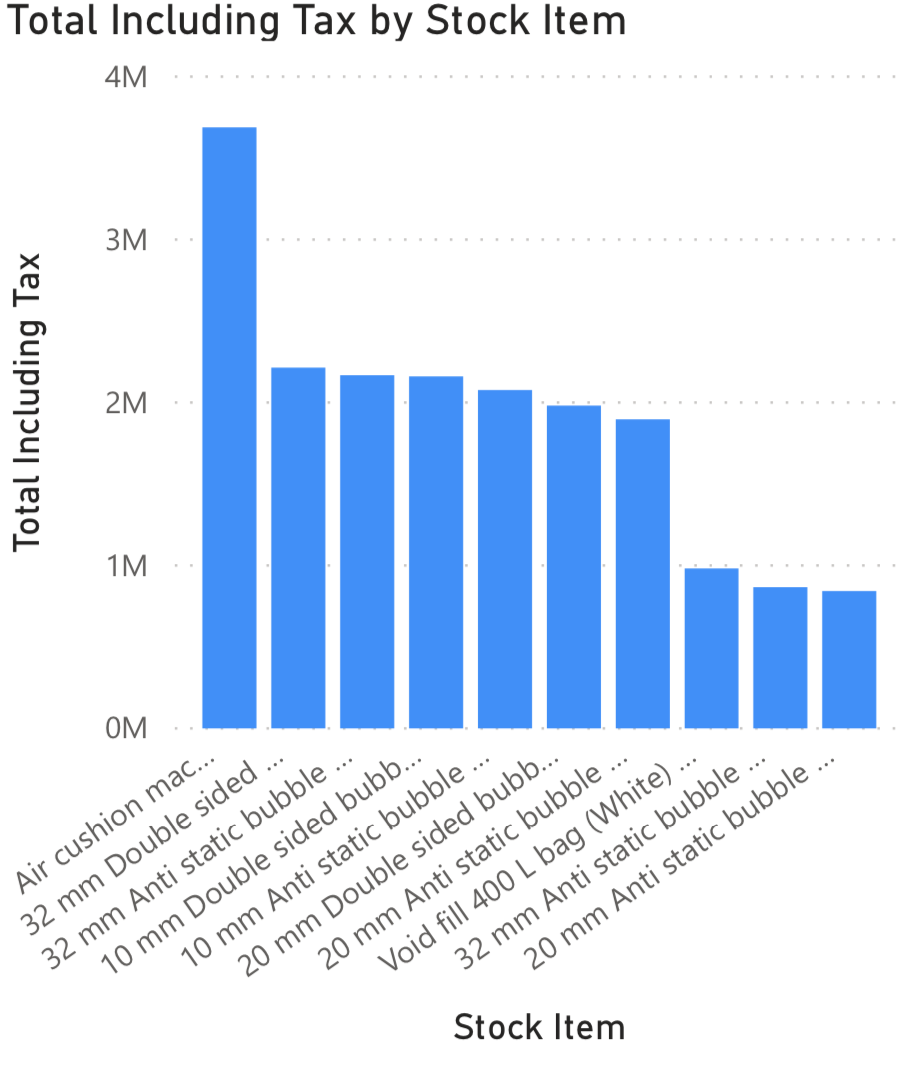
\includegraphics
    {images/Sales/Total Sales By stock item2014.png}
    \caption{Total Sales by item 2014}
    \label{Total Sales by item 2014}
\end{figure}

\begin{figure}[H]
    \centering
    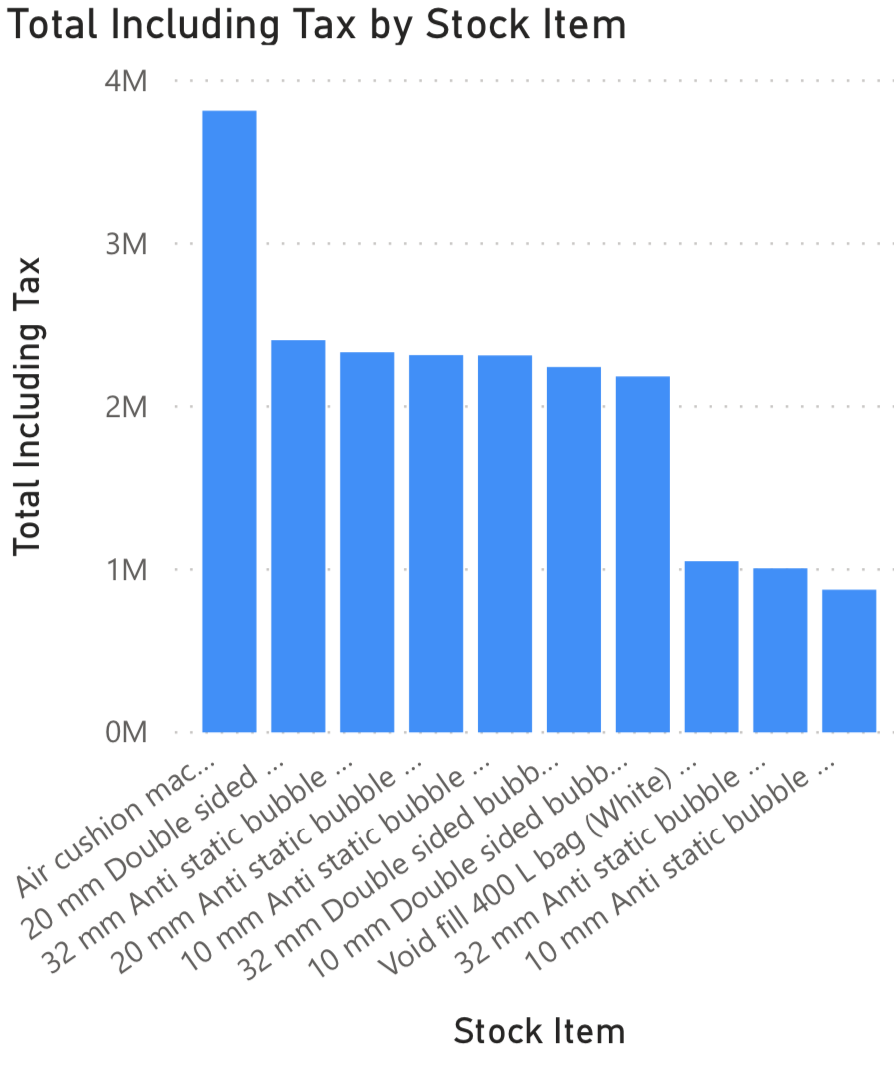
\includegraphics
    {images/Sales/Total Sales By stock item2015.png}
    \caption{Total Sales by item 2015}
    \label{Total Sales by item 2015}
\end{figure}

\begin{figure}[H]
    \centering
    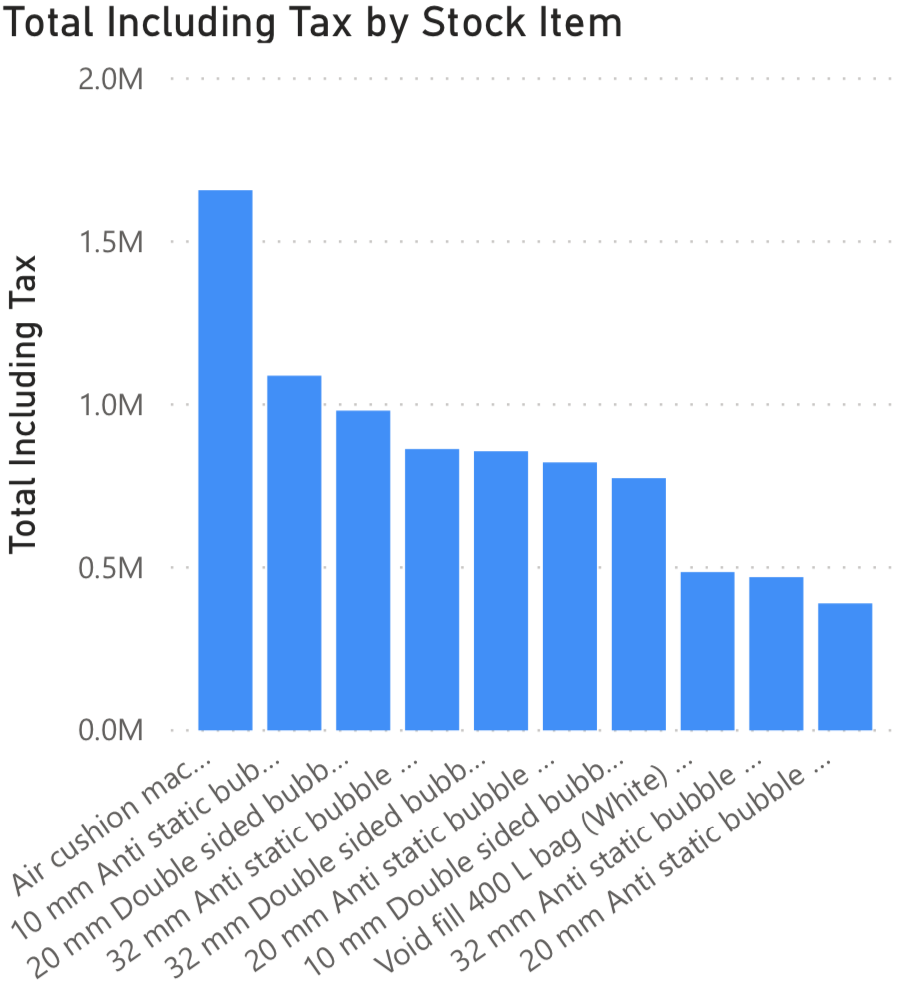
\includegraphics
    {images/Sales/Total Sales By stock item2016.png}
    \caption{Total Sales by item 2016}
    \label{Total Sales by item 2016}
\end{figure}

\begin{figure}[H]
    \centering
    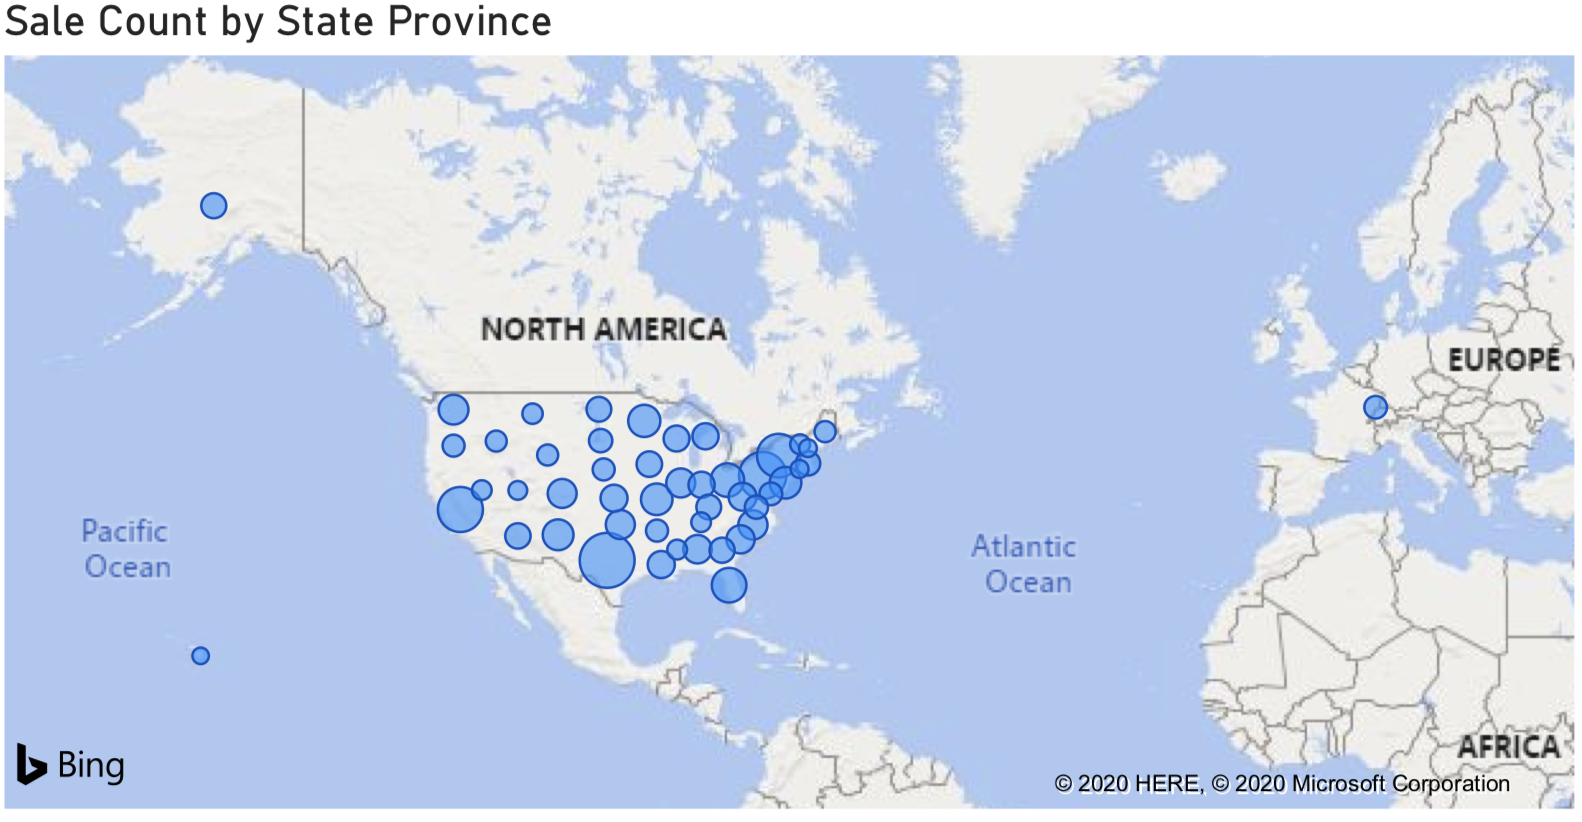
\includegraphics [width=17.5cm]
    {images/Sales/Sale Count by State Province2013.png}
    \caption{Sale Count by State Province2013}
    \label{Sale Count by State Province2013}
\end{figure}









\begin{figure}[H]
    \centering
    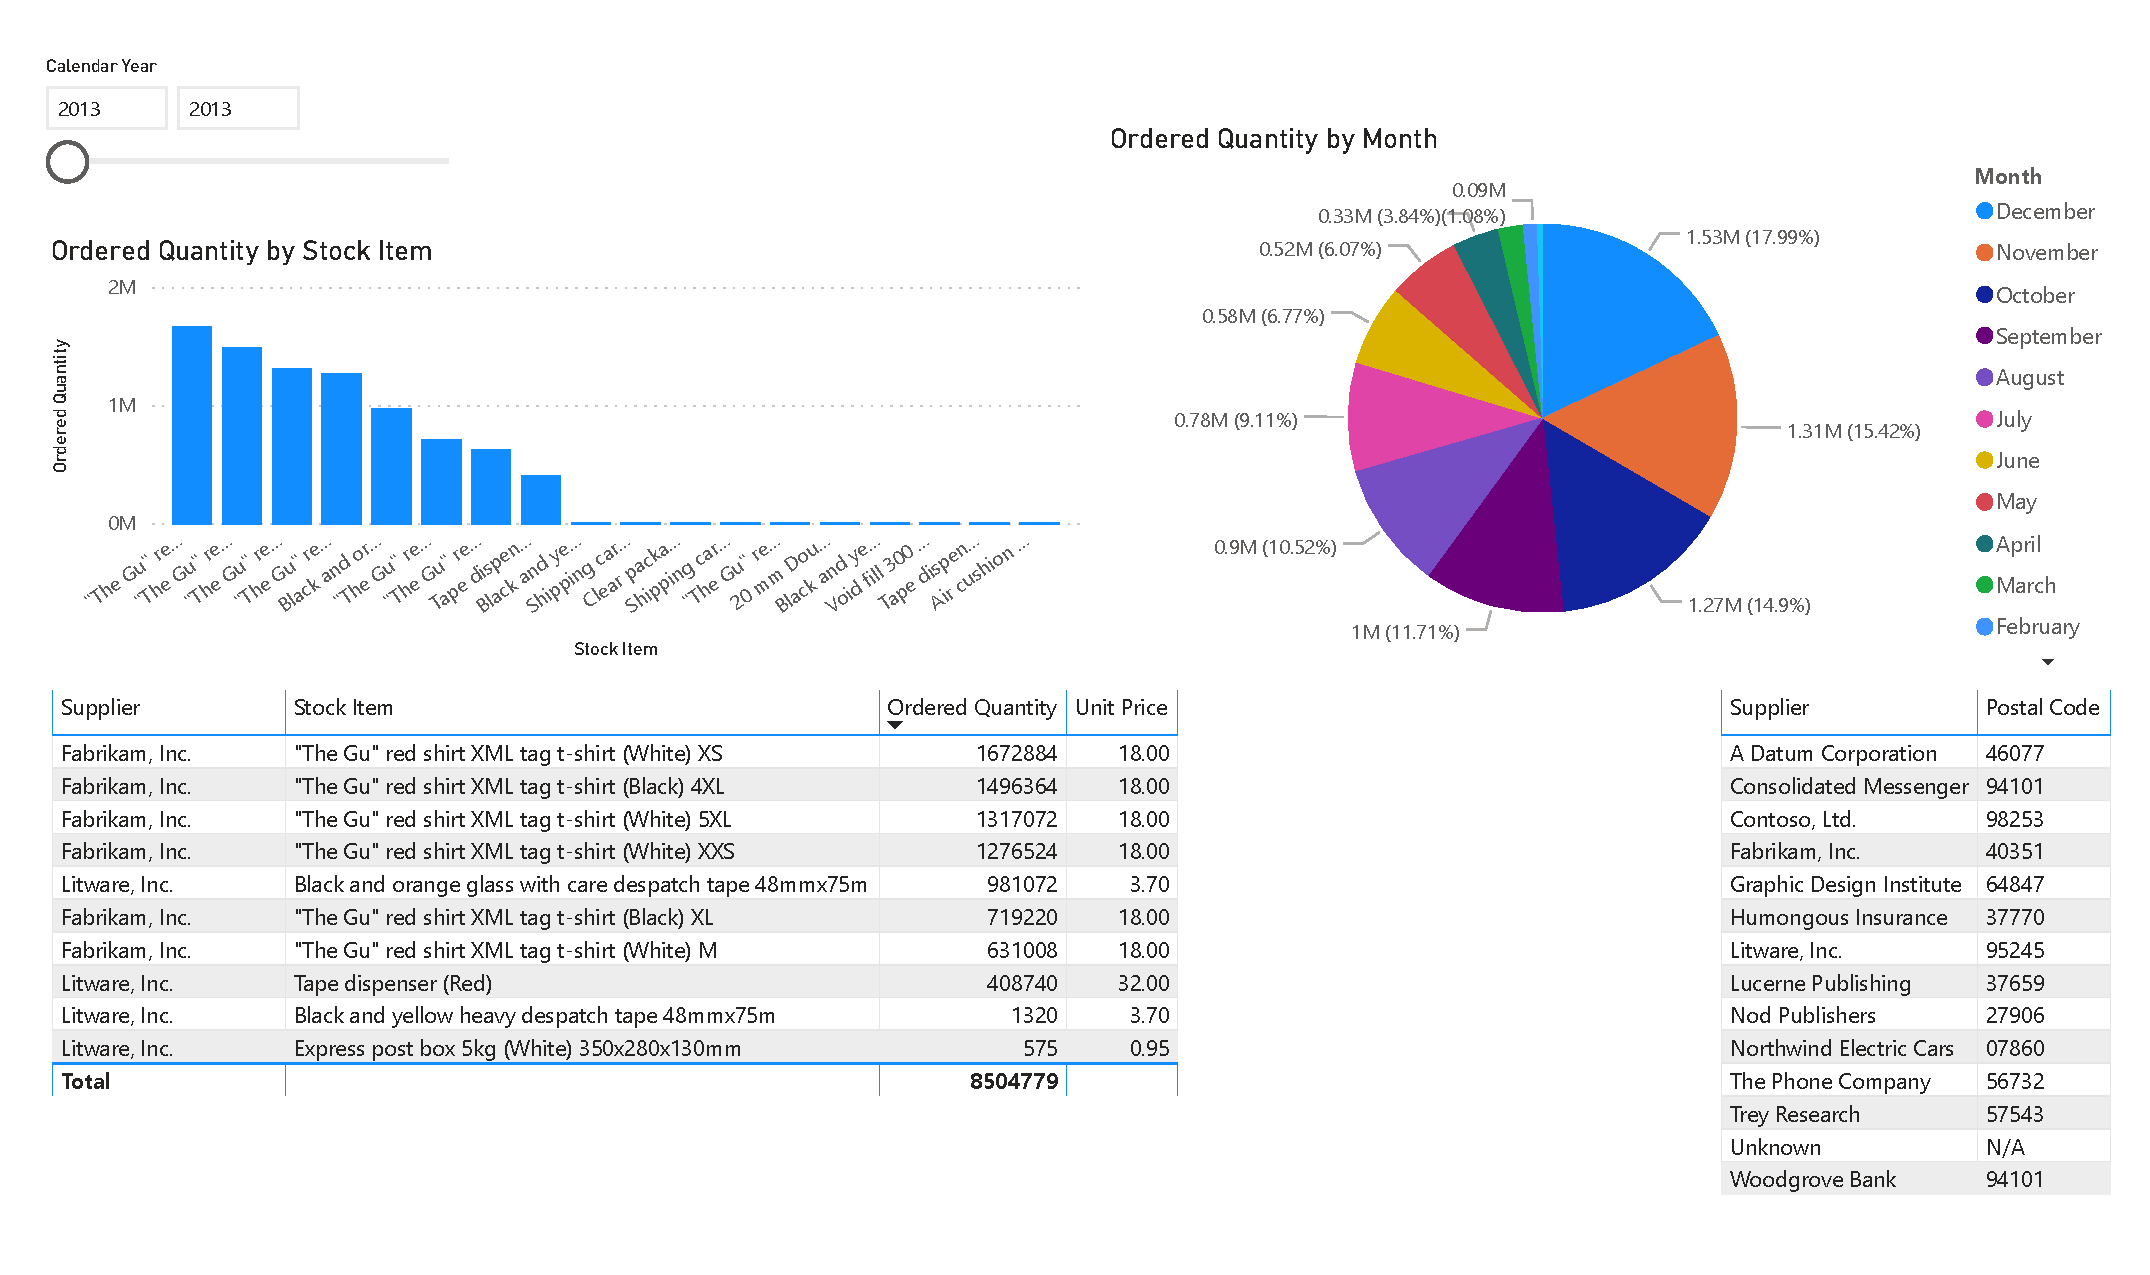
\includegraphics[width=18.5cm, angle=90]
    {images/item Purchase2013.pdf}
    \caption{Item Purchase 2013 DashBoard}
    \label{Item Purchase 2013 DashBoard}
\end{figure}
\begin{figure}[H]
    \centering
    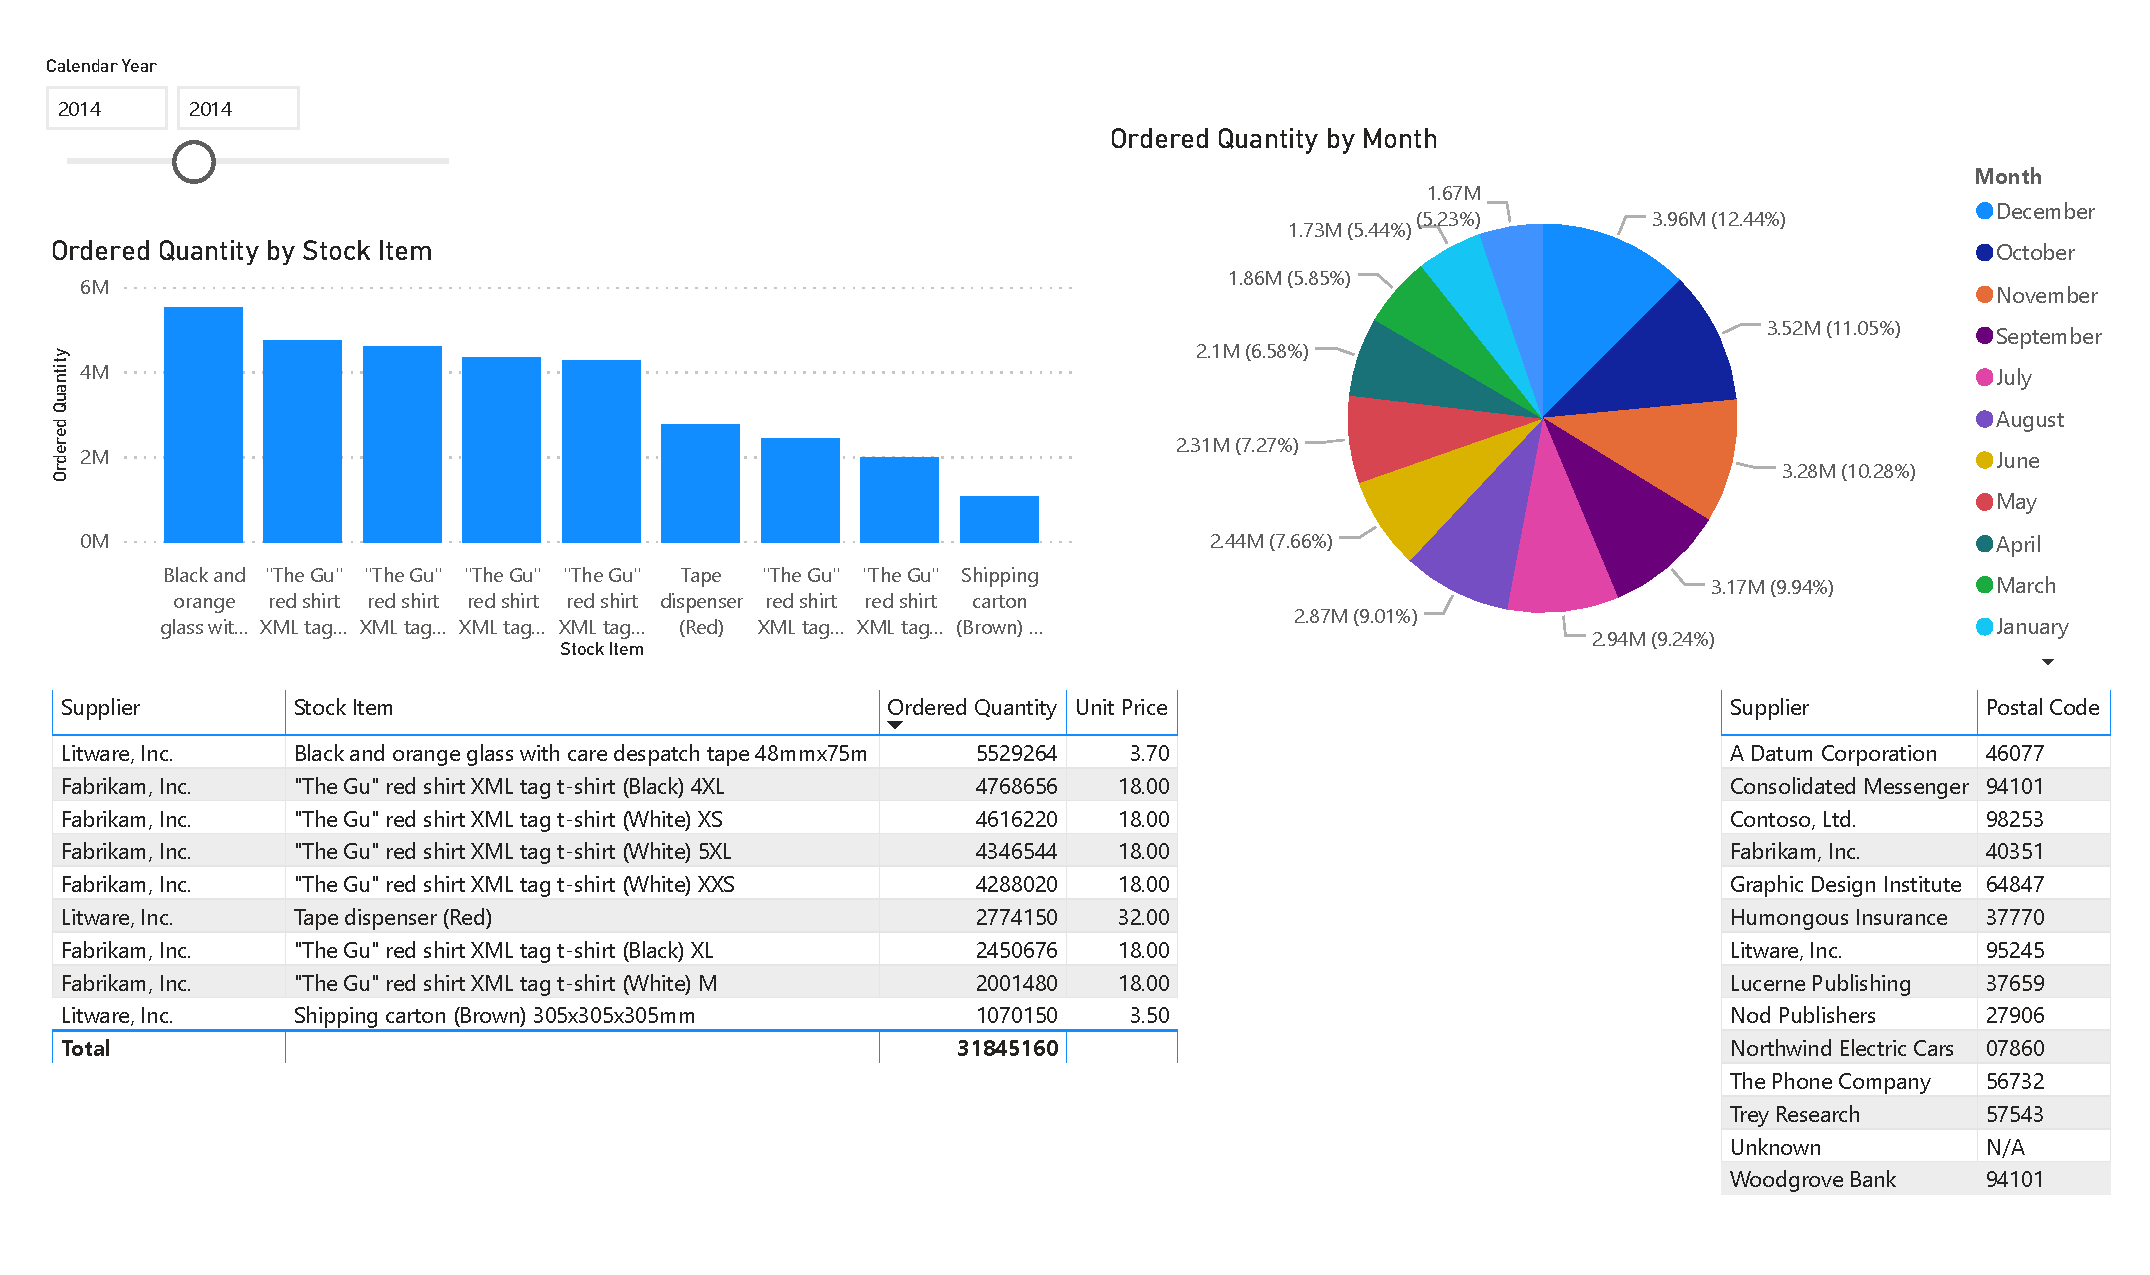
\includegraphics[width=18.5cm, angle=90]
    {images/item Purchase2014.pdf}
    \caption{Item Purchase 2014 DashBoard}
    \label{Item Purchase 2014 DashBoard}
\end{figure}
\begin{figure}[H]
    \centering
    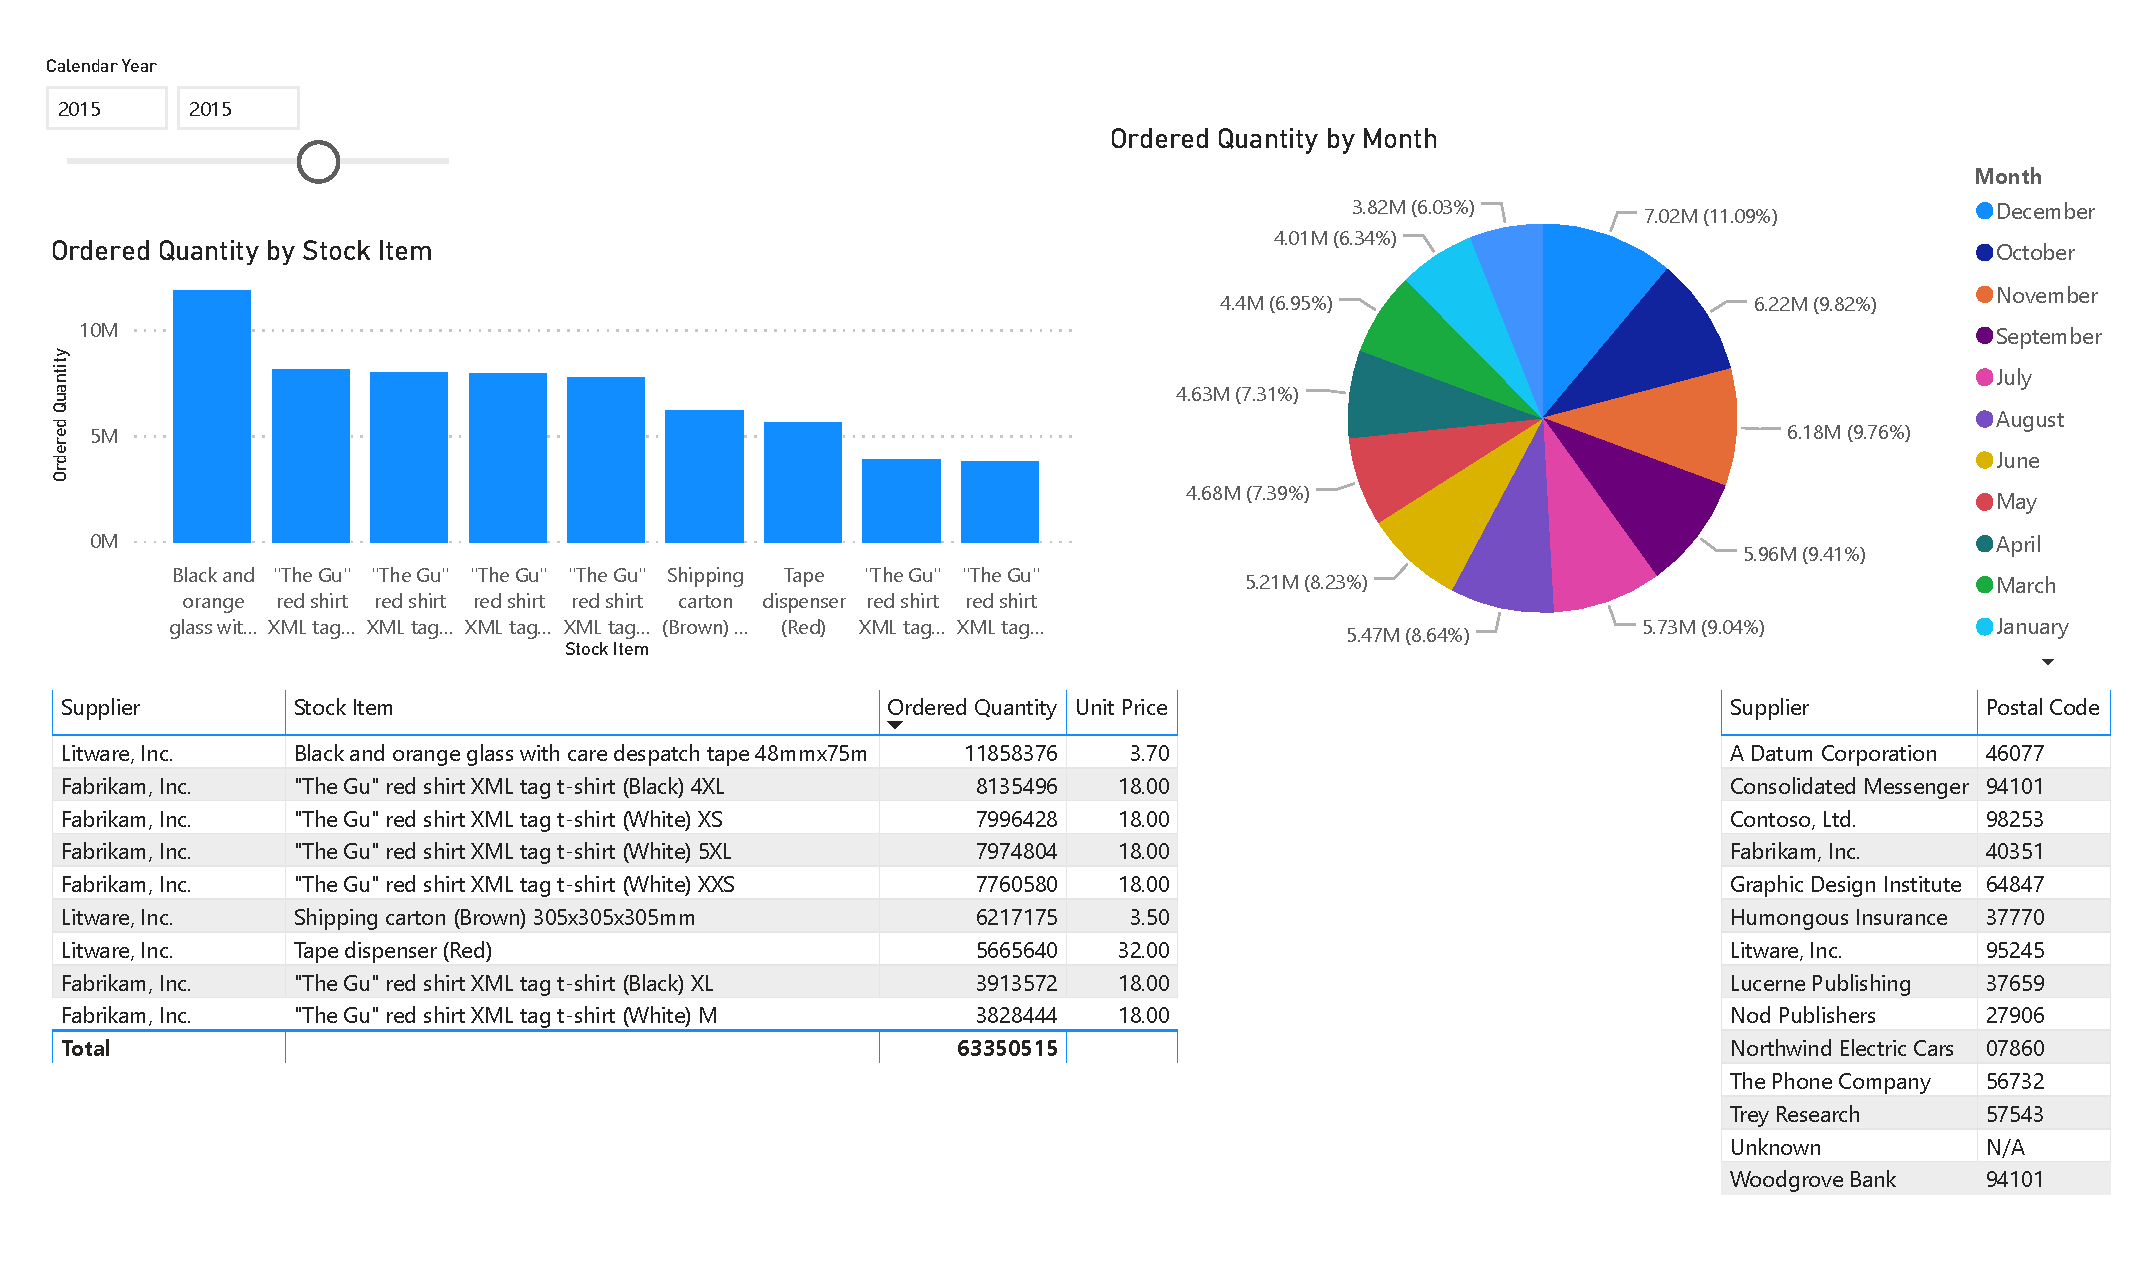
\includegraphics[width=18.5cm, angle=90]
    {images/item Purchase2015.pdf}
    \caption{Item Purchase 2015 DashBoard}
    \label{Item Purchase 2015 DashBoard}
\end{figure}
\begin{figure}[H]
    \centering
    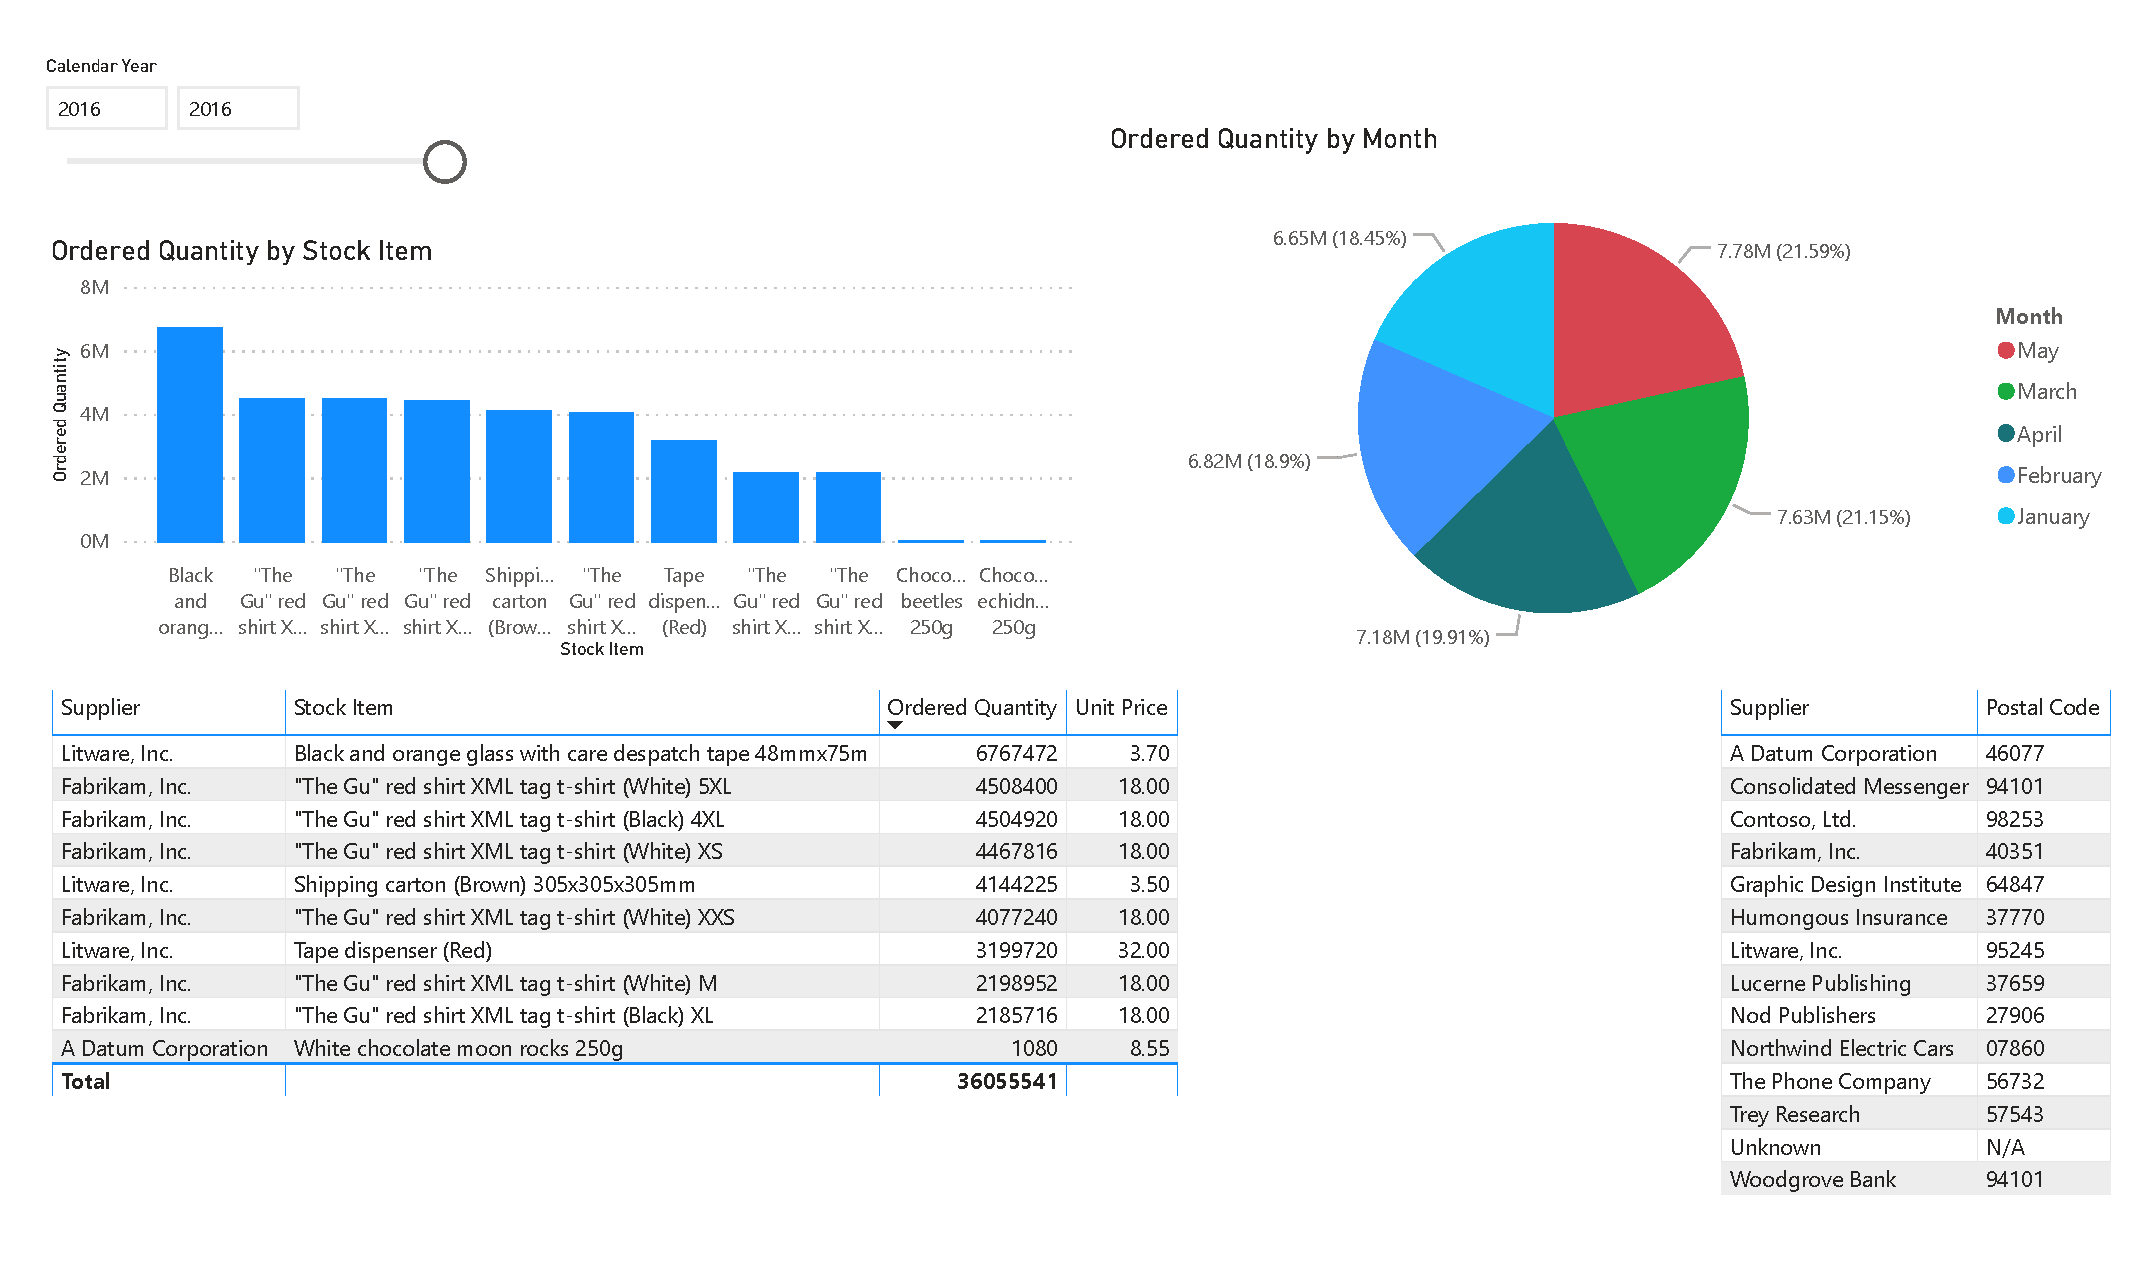
\includegraphics[width=18.5cm, angle=90]
    {images/item Purchase2016.pdf}
    \caption{Item Purchase 2016 DashBoard}
    \label{Item Purchase 2016 DashBoard}
\end{figure}

\end{document}